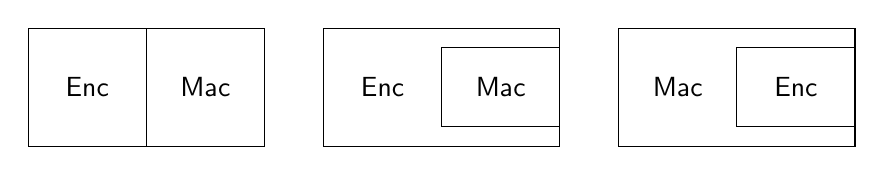
\begin{tikzpicture}
\node (enc1) [minimum width=1.5cm, minimum height=1.5cm, draw] {$\mathsf{Enc}$};
\node (mac1) [right of=enc1, minimum width=1.5cm, minimum height=1.5cm, node distance=1.5cm, draw] {$\mathsf{Mac}$};	

\node (enc2) [right of=mac1, node distance=3cm, minimum width=3cm, minimum height=1.5cm, draw] {};
\node (mac2) [right of=enc2, minimum width=1.5cm, minimum height=1cm, node distance=0.75cm, draw] {$\mathsf{Mac}$};
\node (enc4) [left of=enc2, minimum width=1cm, minimum height=1cm, node distance=0.75cm] {$\mathsf{Enc}$}; 

\node (mac3) [right of=mac2, node distance=3cm, minimum width=3cm, minimum height=1.5cm, draw] {};
\node (enc3) [right of=mac3, minimum width=1.5cm, minimum height=1cm, node distance=0.75cm, draw] {$\mathsf{Enc}$};
\node (enc5) [left of=mac3, minimum width=1cm, minimum height=1cm, node distance=0.75cm] {$\mathsf{Mac}$};	
\end{tikzpicture}